% Provenance (never printed): see sources/outline_sources.md (Year 3:
% stereographic projection; fold and fault analysis; palaeostress; balanced
% cross-sections). Brief: sources/book5/BRIEFS.md, ch. 8. Nets, pi-diagram and
% fault-slip data from figdata/bachelor-3/stereonet.py (Varden data invented,
% from figdata/shared/region.py); Fry plot from figdata/bachelor-3/fry.py.
% Exercise and problem values in the Book 5 scratch calculator calc/ch08.py.
% No real-world numbers: no ledger rows.
\chapter{Análisis estructural}\label{ch:b3:structural-analysis}

Un geólogo ha medido doscientos planos de estratificación en los flancos de un pliegue
demasiado grande para verse entero: su charnela yace bajo un bosque, y sus flancos se extienden a lo largo de
kilómetros. Cada medida es un par de números. Representados como puntos en una carta circular,
los \omterm{def:b3:structural-analysis:stereo}{polos} de los planos caen sobre una única curva, un círculo máximo, y
el \omterm{def:b3:structural-analysis:stereo}{polo} de ese círculo máximo es el eje del pliegue, una recta que nadie ha
llegado a ver jamás. Este capítulo construye la carta, la \omterm{def:b3:structural-analysis:stereo}{proyección estereográfica}, y
la emplea, junto con las herramientas vectoriales que la sustentan, para hallar ejes de pliegue, medir la
deformación registrada por objetos deformados, recuperar el esfuerzo que impulsó un conjunto de
fallas, y restaurar un corte deformado a su estado anterior a la
deformación.

\begin{recall}
Los círculos máximos y los círculos menores de una esfera están en el volumen de primer año, en su capítulo
de astronomía esférica; el rumbo, el buzamiento, la dirección de buzamiento, el acimut y la inmersión en sus
capítulos sobre mapas geológicos y cortes geológicos; la normal unitaria hacia arriba de un
plano de dirección de buzamiento $\alpha$ y buzamiento $\delta$, $\vec n = (\sin\delta
\sin\alpha, \sin\delta\cos\alpha, \cos\delta)$ en componentes este, norte y hacia arriba,
y la media vectorial de un conjunto de medidas en su primer capítulo sobre
métodos de campo y de laboratorio. Los elementos y las clases de pliegues, la línea de charnela de un
pliegue, paralela a $\vec n_1\times\vec n_2$, y el ángulo entre flancos
$\ang{180} - \arccos(\vec n_1\cdot\vec n_2)$, así como la teoría de Anderson del
fallamiento, están en su capítulo sobre fallas, pliegues y fábricas; el esfuerzo, los
esfuerzos principales, la elipse de deformación y la cizalla simple en su capítulo sobre
esfuerzo, deformación y reología; el cabeceo de un vector de deslizamiento (a partir del rumbo,
\ang{-90} para una falla normal, \ang{90} para una falla inversa, 0 sinestral y
\ang{180} dextral) y los ejes P y T de un mecanismo focal en su capítulo sobre
la fuente sísmica. El corte equilibrado y el despegue están en
el volumen de segundo año, en su capítulo sobre los Alpes. Los mínimos cuadrados están en
la \cref{sec:b3:seismology-imaging:inverse}; los autovalores y autovectores de una
matriz simétrica se encuentran en los libros de matemáticas.
\end{recall}

\section{La proyección estereográfica}\label{sec:b3:structural-analysis:stereo}

Los datos de un geólogo son orientaciones: la actitud de un plano de estratificación, de una
falla, de una foliación; el acimut y la inmersión de una lineación, de una charnela de pliegue, de una
dirección de deslizamiento. Cada una es una dirección que pasa por un punto, sin posición. Para
comparar cientos de ellas, conviene imaginarlas todas trasladadas al centro de una misma esfera:
una recta corta la mitad inferior de la esfera en un punto; un plano la corta a lo largo de
un semicírculo máximo. Una carta del hemisferio inferior muestra entonces las rectas como
puntos y los planos como curvas.

\begin{definition}[Proyección estereográfica, red equiangular, proyección equivalente, polo]\label{def:b3:structural-analysis:stereo}
Sea una recta que pasa por el centro $O$ de una esfera de radio $R$ y que corta el
hemisferio inferior en $P$, formando con el nadir el ángulo $\theta = \ang{90} - p$, donde
$p$ es la inmersión de la recta y $t$ su acimut. La
\emph{proyección estereográfica}\index{proyección estereográfica} asigna a $P$ el punto donde la
recta que une el cenit con $P$ corta al plano horizontal que pasa por $O$; ese
punto dista $r$ de $O$ en el acimut $t$. La
carta del hemisferio inferior dibujada de este modo, con su retícula de círculos máximos y
círculos menores, es la \emph{red equiangular}\index{red equiangular} (o
red de Wulff). La \emph{proyección equivalente (de la esfera)}\index{proyección equivalente (de la esfera)}
asigna a $P$ el punto a la distancia $r =
R\sqrt2\sin(\theta/2)$ en el acimut $t$; su red es la red de Schmidt. El
\emph{polo}\index{polo (de un plano)} de un plano es su recta normal, representada como
un punto: para un plano de dirección de buzamiento $\alpha$ y buzamiento $\delta$, el polo
tiene acimut $\alpha + \ang{180}$ e inmersión $\ang{90} - \delta$.
\end{definition}

Ambas proyecciones sitúan una recta vertical en el centro y una recta horizontal sobre
el círculo de radio $R$, la primitiva. Difieren en lo que conservan.

\begin{theorem}[Las dos proyecciones]\label{thm:b3:structural-analysis:projections}
\begin{enumerate}[label=(\alph*)]
  \item La \omterm{def:b3:structural-analysis:stereo}{proyección estereográfica} sitúa $P$ en $r = R\tan(\theta/2)$. Es
        conforme: en cada punto dilata todas las direcciones por el mismo
        factor, $1/(2\cos^2(\theta/2))$, de modo que conserva los ángulos entre
        curvas.
  \item La proyección equivalente multiplica toda área por el mismo factor,
        $1/2$: el área de una región de la red es la mitad del área de la región
        del hemisferio que representa.
\end{enumerate}
\end{theorem}

\begin{proof}
(a) En el plano vertical que pasa por el cenit $Z$, el nadir y $P$
(primera figura de abajo), el arco que va del nadir a $P$
subtiende el ángulo $\theta$ en el centro, de donde el ángulo inscrito
$\theta/2$ en $Z$, que está a la distancia $R$ por encima de $O$: $r =
R\tan(\theta/2)$. Un pequeño paso $R\,\mathrm d\theta$ sobre la esfera hacia el
nadir se convierte en $\mathrm dr = R\,\mathrm d\theta/(2\cos^2(\theta/2))$ en la
carta. El círculo de puntos a ángulo $\theta$ del nadir tiene la
circunferencia $2\pi R\sin\theta$ y se convierte en un círculo de circunferencia $2\pi
r$; la razón es $\tan(\theta/2)/\sin\theta = 1/(2\cos^2(\theta/2))$, la misma
que a lo largo del radio. Una aplicación que dilata igual en dos direcciones perpendiculares
dilata igual en todas las direcciones y conserva los ángulos.

(b) El casquete de la esfera dentro del ángulo $\theta$ del nadir tiene el área
$2\pi R^2(1 - \cos\theta) = 4\pi R^2\sin^2(\theta/2)$; su imagen es el disco
de área $\pi r^2 = 2\pi R^2\sin^2(\theta/2)$, la mitad de aquella. Ambas áreas se
reparten por igual en acimut, de modo que el sector del casquete entre dos acimutes
y su imagen conservan la razón $1/2$, y lo mismo ocurre con el anillo entre dos valores
de $\theta$, diferencia de dos casquetes. Toda región es una unión de tales
sectores anulares pequeños.
\end{proof}

La \omterm{def:b3:structural-analysis:stereo}{proyección estereográfica} transforma además todo círculo de la esfera, máximo o
menor, en un círculo o en una recta de la carta; lo damos por supuesto. Esto hace que la
\omterm{def:b3:structural-analysis:stereo}{red equiangular} sea fácil de trazar con compás, y un círculo menor, el cono de las rectas que
forman un ángulo fijo con un eje, conserva su forma. La proyección equivalente
deforma las formas: un círculo menor se convierte en un óvalo, estirado
alrededor de la primitiva. Es la proyección en la que una nube de \omterm{def:b3:structural-analysis:stereo}{polos} puede
contarse, puesto que una misma área de la red contiene una misma parte de las
direcciones del hemisferio; los geólogos estructurales, y los sismólogos para sus
mecanismos focales, la emplean para sus datos.

\begin{omfigure}
\begin{tikzpicture}[scale=1.0, >=stealth]
% (a) equal-angle: theta = 60 deg, R = 2 cm; r = 2 tan 30 = 1.155
\begin{scope}
\draw[thick] (0,0) circle (2);
 \draw (-2.5,0) -- (2.5,0) node[right, font=\scriptsize] {plano};
 \fill (0,2) circle (1.5pt) node[above, font=\scriptsize] {cenit $Z$};
 \fill (0,-2) circle (1.5pt) node[below, font=\scriptsize] {nadir};
\fill (0,0) circle (1.2pt) node[above left, font=\scriptsize] {$O$};
\draw[dashed] (0,2) -- (0,-2);
\draw[omDef, thick] (0,0) -- (1.732,-1);
\fill[omDef] (1.732,-1) circle (1.5pt) node[below right, font=\scriptsize] {$P$};
\draw[omThm] (0,2) -- (1.732,-1);
\fill[omThm] (1.155,0) circle (1.5pt);
\node[omThm, font=\scriptsize, above right] at (1.155,0) {$P'$};
\draw (0,-0.6) arc[start angle=-90, end angle=-30, radius=0.6];
\node[font=\scriptsize] at (0.38,-0.85) {$\theta$};
\draw (0,1.2) arc[start angle=-90, end angle=-60, radius=0.8];
\node[font=\scriptsize] at (0.25,0.95) {$\theta/2$};
\draw[<->] (0,0.25) -- (1.155,0.25);
\node[font=\scriptsize, above] at (0.58,0.25) {$r$};
 \node[font=\small] at (0,-3.0) {(a) equiangular};
\end{scope}
% (b) equal-area: chord from nadir to P = 2R sin(theta/2) = 2
\begin{scope}[xshift=6.6cm]
\draw[thick] (0,0) circle (2);
\draw (-2.5,0) -- (2.5,0);
 \draw (-2.5,-2) -- (2.5,-2) node[right, font=\scriptsize] {plano tangente};
 \fill (0,-2) circle (1.5pt) node[below left, font=\scriptsize] {nadir};
\fill (0,0) circle (1.2pt) node[above left, font=\scriptsize] {$O$};
\draw[dashed] (0,2) -- (0,-2);
\draw[omDef, thick] (0,0) -- (1.732,-1);
\fill[omDef] (1.732,-1) circle (1.5pt) node[above right, font=\scriptsize] {$P$};
\draw[omThm] (0,-2) -- (1.732,-1);
\draw[omThm, dashed] (1.732,-1) arc[start angle=30, end angle=0, radius=2];
\fill[omThm] (2,-2) circle (1.5pt);
\node[omThm, font=\scriptsize, below] at (2,-2.05) {$2R\sin(\theta/2)$};
\draw (0,-0.6) arc[start angle=-90, end angle=-30, radius=0.6];
\node[font=\scriptsize] at (0.38,-0.85) {$\theta$};
 \node[font=\small] at (0,-3.0) {(b) equivalente};
\end{scope}
\end{tikzpicture}

\par\smallskip{\small Las dos proyecciones, en el plano vertical que pasa por la
recta $OP$. (a) La \omterm{def:b3:structural-analysis:stereo}{proyección estereográfica} lleva $P$ a $P'$, donde la
recta que parte del cenit corta el plano horizontal: el ángulo en $Z$ es
$\theta/2$, por lo que $r = R\tan(\theta/2)$. (b) La proyección equivalente lleva
$P$, alrededor del nadir, sobre el plano tangente a la distancia $2R\sin(\theta/2)$
de la cuerda; la carta se reescala entonces por $1/\sqrt2$ para que las
rectas horizontales caigan sobre una primitiva de radio $R$.}\label{fig:b3:structural-analysis:geometry}
\end{omfigure}

\begin{omfigure}
\begin{tikzpicture}
\begin{groupplot}[group style={group size=2 by 1, horizontal sep=0.8cm},
  width=0.5\linewidth, height=0.5\linewidth, axis equal image, hide axis,
  xmin=-1.15, xmax=1.15, ymin=-1.15, ymax=1.15, unbounded coords=jump,
  title style={font=\small}]
\nextgroupplot[title={(a) red equiangular (Wulff)}]
% computed in figdata/bachelor-3/stereonet.py
\addplot[gray!75, very thin] table[x=x, y=y] {figdata/out/bachelor-3-stereonet-wulff.dat};
\addplot[gray!75, very thin] coordinates {(-1,0) (1,0)};
\addplot[black, thick, domain=0:360, samples=181] ({cos(x)}, {sin(x)});
\node[font=\scriptsize, above] at (axis cs:0,1.0) {N};
\nextgroupplot[title={(b) red equivalente (Schmidt)}]
\addplot[gray!75, very thin] table[x=x, y=y] {figdata/out/bachelor-3-stereonet-schmidt.dat};
\addplot[gray!75, very thin] coordinates {(-1,0) (1,0)};
\addplot[black, thick, domain=0:360, samples=181] ({cos(x)}, {sin(x)});
\node[font=\scriptsize, above] at (axis cs:0,1.0) {N};
\end{groupplot}
\end{tikzpicture}

\par\smallskip{\small Las dos redes, trazadas a partir de las fórmulas del teorema
anterior: círculos máximos de los planos de rumbo norte--sur que buzan cada
\ang{10} hacia el este y el oeste, y círculos menores cada \ang{10} alrededor del
eje norte--sur. En la \omterm{def:b3:structural-analysis:stereo}{red equiangular} los círculos menores son círculos; en la
red equivalente son óvalos, pero las áreas iguales contienen partes iguales de las
direcciones.}\label{fig:b3:structural-analysis:nets}
\end{omfigure}

\paragraph{Planos, rectas y ángulos.}
Un plano de dirección de buzamiento $\alpha$ y buzamiento $\delta$ corta el hemisferio inferior
según un semicírculo máximo. Sus extremos están sobre la primitiva, en los dos extremos
del rumbo; su punto medio es la línea de máxima pendiente, que se inclina $\delta$
hacia $\alpha$; y su \omterm{def:b3:structural-analysis:stereo}{polo} dista \ang{90} de cada punto suyo, en el
acimut $\alpha + \ang{180}$. Una recta contenida en el plano es un punto del
círculo máximo. Para representar los datos, se coloca sobre la red una lámina transparente que se gira
alrededor del centro hasta que el rumbo de los datos quede sobre el diámetro norte--sur de la red;
se traza entonces el círculo máximo del buzamiento correspondiente, y la lámina se
devuelve a su posición. El ángulo entre dos rectas se mide sobre el círculo máximo que pasa
por ambos puntos, contando las divisiones de los círculos menores que cruza, tras
girar la lámina hasta que ambos puntos queden sobre un mismo círculo máximo de la red. El
ángulo entre dos planos es el ángulo entre sus \omterm{def:b3:structural-analysis:stereo}{polos}, o su suplementario.
Un ordenador hace lo mismo con vectores: el ángulo entre dos rectas de vectores unitarios
$\vec u$ y $\vec v$ es $\arccos|\vec u\cdot\vec v|$.

\begin{method}[Rotación de datos alrededor de un eje]\label{met:b3:structural-analysis:rotation}
Para deshacer un basculamiento, por ejemplo para devolver un estrato a la horizontal con las
lineaciones que lleva, o para restituir una dirección paleomagnética medida
en estratos basculados (véase el \cref{ch:b3:palaeomagnetism}):
\begin{enumerate}
  \item Elíjase el eje de rotación: para un estrato basculado, su línea de rumbo,
        horizontal; el ángulo es el buzamiento, en el sentido que lleva el estrato hacia arriba.
  \item Sobre la red, se gira la lámina hasta que el eje quede a lo largo del
        diámetro norte--sur, donde los círculos menores son los conos alrededor
        de él.
  \item Se desplaza cada punto a lo largo de su círculo menor un ángulo igual al de rotación,
        medido sobre los círculos máximos. Un punto que saliera del hemisferio
        inferior reaparece en el extremo opuesto de su círculo menor, en el
        acimut opuesto.
  \item Se devuelve la lámina a su posición. Con vectores, la rotación de $\vec v$ según el
        ángulo $\omega$ alrededor del eje unitario $\vec k$ es $\vec v' = \vec v
        \cos\omega + (\vec k\times\vec v)\sin\omega + \vec k(\vec k\cdot\vec
        v)(1 - \cos\omega)$.
\end{enumerate}
\end{method}

\section{Análisis de pliegues}\label{sec:b3:structural-analysis:folds}

Un pliegue cilíndrico se genera por una recta, el eje de pliegue, desplazada
paralelamente a sí misma. Todo plano tangente a la superficie plegada contiene el
eje, de modo que toda normal a la superficie es perpendicular al eje: todos los
\omterm{def:b3:structural-analysis:stereo}{polos} se sitúan sobre el círculo máximo del plano perpendicular al eje.

\begin{definition}[Diagrama pi, eje beta]\label{def:b3:structural-analysis:pi}
El \emph{diagrama pi}\index{diagrama pi} de un pliegue es la representación de los \omterm{def:b3:structural-analysis:stereo}{polos} de
los planos medidos sobre su superficie plegada. Para un pliegue cilíndrico caen sobre
un círculo máximo, la faja $\pi$; el \omterm{def:b3:structural-analysis:stereo}{polo} de la faja es el
\emph{eje beta}\index{eje beta}, la estimación del eje de pliegue que dan las
medidas.
\end{definition}

Con solo dos flancos, el \omterm{def:b3:structural-analysis:pi}{eje beta} es el producto vectorial de sus normales, como
mostró el volumen de primer año para la línea de charnela. Con doscientas lecturas dispersas
lecturas, hace falta un ajuste óptimo. La media vectorial, que sirvió para las lecturas
de un solo plano, no sirve: los \omterm{def:b3:structural-analysis:stereo}{polos} de una faja apuntan en todos los sentidos a lo largo de ella, y
su media dice poco del círculo sobre el que se sitúan.

\begin{definition}[Tensor de orientación]\label{def:b3:structural-analysis:orientation-tensor}
El \emph{tensor de orientación}\index{tensor de orientación} de $N$ vectores unitarios
$\vec p_1, \dots, \vec p_N$ es la matriz simétrica
\[
  T = \frac1N\sum_{i=1}^N \vec p_i\,\vec p_i^{\mathsf T},
  \qquad T_{jk} = \frac1N\sum_i p_{ij}\,p_{ik} .
\]
No cambia cuando un vector se sustituye por su opuesto, por lo que resulta adecuado para
ejes y \omterm{def:b3:structural-analysis:stereo}{polos}, que carecen de sentido. Sus valores propios $\lambda_1 \ge \lambda_2
\ge \lambda_3 \ge 0$ suman la traza, $1$.
\end{definition}

\begin{theorem}[Agrupamiento y faja a partir del tensor de orientación]\label{thm:b3:structural-analysis:tensor}
Para cualquier vector unitario $\vec u$,
\[
  \frac1N\sum_{i=1}^N (\vec p_i\cdot\vec u)^2 = \vec u^{\mathsf T}T\,\vec u ,
\]
que alcanza su valor mínimo, $\lambda_3$, cuando $\vec u$ es el vector propio
$\vec e_3$ del valor propio menor, y su máximo, $\lambda_1$, a lo largo del
vector propio $\vec e_1$. Como $\vec p_i\cdot\vec u$ es el seno del ángulo
entre $\vec p_i$ y el plano perpendicular a $\vec u$, el círculo máximo
perpendicular a $\vec e_3$ es la faja que minimiza la suma de los cuadrados
de los senos de las distancias de los \omterm{def:b3:structural-analysis:stereo}{polos} a ella, y $\sqrt{\lambda_3}$ es la
raíz cuadrática media de los senos. El eje $\vec e_1$ es la recta más próxima a los vectores,
el eje medio de un agrupamiento.
\end{theorem}

\begin{proof}
$(\vec p_i\cdot\vec u)^2 = \vec u^{\mathsf T}\vec p_i\,\vec p_i^{\mathsf T}\vec
u$; se promedia sobre $i$. La matriz $T$ es simétrica, por lo que tiene una base ortonormal
de vectores propios, en la que $\vec u = \sum_k u_k\vec e_k$ con $\sum_k
u_k^2 = 1$ y $\vec u^{\mathsf T}T\vec u = \sum_k\lambda_k u_k^2$. Es una
media ponderada de los valores propios, con pesos $u_k^2$ que suman 1: así
queda entre $\lambda_3$ y $\lambda_1$, y los alcanza para $\vec u = \vec
e_3$ y $\vec e_1$.
\end{proof}

Los valores propios describen la forma de los datos. Un agrupamiento tiene $\lambda_1$ cercano a
1 y los otros dos pequeños; una faja tiene $\lambda_3$ cercano a 0, al estar repartidos los \omterm{def:b3:structural-analysis:stereo}{polos}
a lo largo del círculo, de modo que $\lambda_1$ y $\lambda_2$ reparten el resto;
los vectores dispersos uniformemente dan tres valores propios cercanos a $1/3$. Un pliegue es
cilíndrico, dentro de la precisión de las lecturas, cuando $\sqrt{\lambda_3}$ no es
mayor que la dispersión de las lecturas repetidas de un mismo plano. Un pliegue cónico,
o dos generaciones de pliegues, dispersan los \omterm{def:b3:structural-analysis:stereo}{polos} apartándolos de cualquier círculo máximo
y aumentan $\lambda_3$.

La figura siguiente representa doce lecturas de los dos flancos del
anticlinal de Varden, pliegue inventado de la serie (el \cref{pb:b3:structural-analysis:1}
calcula su eje). Los \omterm{def:b3:structural-analysis:stereo}{polos} de los flancos suaves se agrupan cerca del centro de
la red en dos grupos, que juntos definen una faja que discurre casi
este--oeste; el \omterm{def:b3:structural-analysis:pi}{eje beta} se sitúa sobre el primitivo, prácticamente hacia el norte. Los planos medios
de los dos flancos, dibujados como círculos máximos, se cortan en el mismo punto:
el \omterm{def:b3:structural-analysis:pi}{eje beta} es la recta común a todos los flancos.

\begin{omfigure}
\begin{tikzpicture}
\begin{groupplot}[group style={group size=2 by 1, horizontal sep=1.0cm},
  width=0.5\linewidth, height=0.5\linewidth, axis equal image,
  unbounded coords=jump, title style={font=\small}]
\nextgroupplot[hide axis, xmin=-1.15, xmax=1.15, ymin=-1.15, ymax=1.15,
  title={(a) hemisferio inferior}]
% computed in figdata/bachelor-3/stereonet.py (Varden readings invented)
\addplot[gray!35, very thin] table[x=x, y=y] {figdata/out/bachelor-3-stereonet-schmidt.dat};
\addplot[black, thick, domain=0:360, samples=181] ({cos(x)}, {sin(x)});
\addplot[gray, densely dashed] table[x=x, y=y] {figdata/out/bachelor-3-stereonet-limbs.dat};
\addplot[omDef, thick] table[x=x, y=y] {figdata/out/bachelor-3-stereonet-girdle.dat};
\addplot[only marks, mark=*, mark size=1.2pt] table[x=x, y=y] {figdata/out/bachelor-3-stereonet-poles.dat};
\addplot[only marks, mark=triangle*, mark size=3pt, omThm] table[x=x, y=y] {figdata/out/bachelor-3-stereonet-beta.dat};
\node[font=\scriptsize, above] at (axis cs:0,1.02) {N};
\node[omThm, font=\scriptsize, right] at (axis cs:0.06,0.88) {$\beta$};
\draw[gray] (axis cs:-0.3,-0.3) rectangle (axis cs:0.3,0.3);
\nextgroupplot[xmin=-0.3, xmax=0.3, ymin=-0.3, ymax=0.3, title={(b) el centro, ampliado},
  xtick=\empty, ytick=\empty]
\addplot[gray!35, very thin] table[x=x, y=y] {figdata/out/bachelor-3-stereonet-schmidt.dat};
\addplot[omDef, thick] table[x=x, y=y] {figdata/out/bachelor-3-stereonet-girdle.dat};
\addplot[only marks, mark=*, mark size=1.5pt] table[x=x, y=y] {figdata/out/bachelor-3-stereonet-poles.dat};
\node[font=\scriptsize, align=center] at (axis cs:0.16,0.09) {polos del\\ flanco oeste};
\node[font=\scriptsize, align=center] at (axis cs:-0.16,0.09) {polos del\\ flanco este};
\node[omDef, font=\scriptsize] at (axis cs:0.17,-0.06) {$\pi$-faja};
\end{groupplot}
\end{tikzpicture}

\par\smallskip{\small \omterm{def:b3:structural-analysis:pi}{Diagrama pi} del anticlinal de Varden sobre la red equivalente,
hemisferio inferior: los \omterm{def:b3:structural-analysis:stereo}{polos} de doce lecturas de estratificación (puntos), la
faja de mejor ajuste obtenida del \omterm{def:b3:structural-analysis:orientation-tensor}{tensor de orientación} (azul), los círculos máximos de los
dos flancos medios (trazo discontinuo) y el \omterm{def:b3:structural-analysis:pi}{eje beta} (triángulo), donde se cortan los tres
círculos máximos. Un estrato que buza hacia el este tiene su \omterm{def:b3:structural-analysis:stereo}{polo} al oeste del
centro.}\label{fig:b3:structural-analysis:pi}
\end{omfigure}

\section{Análisis de la deformación finita}\label{sec:b3:structural-analysis:strain}

Una roca deformada registra su deformación cuando contiene objetos cuya
forma original, o cuya disposición original, se conoce: ooides redondeados y
manchas de reducción, fósiles de simetría conocida, cantos rodados o
simplemente los centros de granos que en su día estuvieron espaciados de manera uniforme.

\begin{definition}[Análisis de la deformación finita, método de Fry]\label{def:b3:structural-analysis:strain-analysis}
El \emph{análisis de la deformación finita}\index{análisis de la deformación finita} es la medición
de la elipse, o del elipsoide, de deformación que ha sufrido una roca, a partir de las
formas, orientaciones o espaciados de objetos cuyo estado anterior a la
deformación se conoce. En el \emph{método de Fry}\index{método de Fry}, el vector
que va desde el centro de cada objeto hasta el centro de cualquier otro se representa desde
un origen común; cuando los centros estaban dispersos con una separación mínima y sin
dirección preferente, la región vacía alrededor del origen es una elipse de la
forma y orientación de la elipse de deformación.
\end{definition}

\begin{proposition}[El vacío de Fry]\label{prop:b3:structural-analysis:fry}
Si una deformación homogénea transforma cada vector $\vec d$ en $F\vec d$, y ningún par de
centros distaba menos de $d_0$ antes de la deformación, entonces, después de ella, la región
alrededor del origen del diagrama de Fry que está libre de puntos contiene la elipse
$\{F\vec d : |\vec d| < d_0\}$, de semiejes $S_1d_0$ y $S_2d_0$ a lo largo de las
direcciones principales de la deformación.
\end{proposition}

\begin{proof}
Una deformación homogénea desplaza cada punto mediante la misma aplicación lineal, más una
traslación, de modo que la diferencia de dos centros pasa a ser $F\vec d$. Antes de la
deformación, ninguna diferencia se encontraba en el disco de radio $d_0$; después, ninguna se encuentra en
su imagen, que es la elipse de deformación del volumen de primer año escalada por $d_0$.
\end{proof}

En la práctica, los centros no están todos a la separación mínima, y el vacío se
lee como el borde interior del anillo más denso de puntos; su razón estima la
razón de deformación $R_s = S_1/S_2$ algo baja. La figura siguiente pone a prueba el método sobre
una lámina delgada inventada, deformada hasta $R_s = 2$ con el eje largo a
\ang{30} de la horizontal: la elipse ajustada al borde del vacío da
$R_s = 1.9$ y \ang{30}. Cuando se miden los propios objetos, los inicialmente
redondos se convierten en elipses de razón axial $R_s$ exactamente; los inicialmente
elípticos, con orientaciones al azar, terminan con razones $R_f$ dispersas
en torno a $R_s$, siendo los valores mayores cuando sus ejes largos partían paralelos a la
dirección de estiramiento, y sus orientaciones finales $\varphi$ se agrupan en torno a
ella. La representación de $R_f$ frente a $\varphi$, leída con tablas o con un ordenador,
separa la deformación de las formas originales.

\begin{omfigure}
\begin{tikzpicture}
\begin{groupplot}[group style={group size=2 by 1, horizontal sep=1.2cm},
  width=0.5\linewidth, height=0.5\linewidth, axis equal image,
  title style={font=\small}, tick label style={font=\scriptsize}]
\nextgroupplot[xmin=-10, xmax=10, ymin=-10, ymax=10, title={(a) centros de grano tras la deformación}]
% computed in figdata/bachelor-3/fry.py (invented population)
\addplot[only marks, mark=o, mark size=1.6pt, black] table[x=x, y=y] {figdata/out/bachelor-3-fry-points.dat};
\nextgroupplot[xmin=-2.6, xmax=2.6, ymin=-2.6, ymax=2.6, title={(b) diagrama de Fry}]
\addplot[only marks, mark=*, mark size=0.5pt, black] table[x=x, y=y] {figdata/out/bachelor-3-fry-fry.dat};
\addplot[omThm, thick] table[x=x, y=y] {figdata/out/bachelor-3-fry-fit.dat};
\end{groupplot}
\end{tikzpicture}

\par\smallskip{\small El \omterm{def:b3:structural-analysis:strain-analysis}{método de Fry} sobre una población inventada de centros de grano,
dispuestos con una separación mínima de 1 y deformados después hasta $R_s = 2$,
con el eje largo a \ang{30} en sentido antihorario desde la horizontal, conservando el área. (a) Los
centros, en los que apenas se aprecia la deformación a simple vista. (b) Los vectores entre todos los
pares de centros separados menos de 2.6: el centro vacío es la elipse de deformación. La
elipse roja se ajusta al punto más cercano en cada uno de los 36 sectores: razón 1.9,
eje largo a \ang{30}.}\label{fig:b3:structural-analysis:fry}
\end{omfigure}

En tres dimensiones, el elipsoide de deformación tiene los estiramientos principales $X \ge Y
\ge Z$. Su forma se representa en el diagrama de Flinn, con $a = X/Y$ frente a $b =
Y/Z$ y el parámetro
\[
  k = \frac{a - 1}{b - 1} .
\]
Sobre la recta $k = 1$, que corresponde a la deformación plana a volumen constante ($Y = 1$,
$X = 1/Z$, de modo que $a = b$), el elipsoide no es ni alargado en forma de puro ni aplastado en forma de torta. Por encima,
$k > 1$, el elipsoide es prolato, estirado en una dirección por una
constricción: las rocas deformadas de este modo desarrollan una lineación marcada. Por debajo, $k < 1$,
es oblato, aplastado, y la roca desarrolla una foliación marcada.

\begin{omfigure}
\begin{tikzpicture}[scale=1.0, >=stealth]
\draw[->] (0,0) -- (5.4,0) node[right, font=\scriptsize] {$b = Y/Z$};
\draw[->] (0,0) -- (0,4.6) node[above, font=\scriptsize] {$a = X/Y$};
\foreach \v/\l in {0/1, 1.5/2, 3/3, 4.5/4} {
  \draw (\v,0) -- (\v,-0.08) node[below, font=\scriptsize] {\l};
  \draw (0,\v) -- (-0.08,\v) node[left, font=\scriptsize] {\l};
}
\draw[omDef, thick] (0,0) -- (4.5,4.5) node[right, font=\scriptsize, align=left] {$k = 1$\\ deformación plana};
\node[font=\scriptsize, align=center] at (1.3,3.6) {constricción\\ $k > 1$, prolato};
\node[font=\scriptsize, align=center] at (4.3,1.1) {aplastamiento\\ $k < 1$, oblato};
% shapes
\draw[fill=omLithLime] (0.9,2.75) ellipse (0.55 and 0.12);
\draw[fill=omLithLime] (4.3,2.1) ellipse (0.45 and 0.22);
\end{tikzpicture}

\par\smallskip{\small El diagrama de Flinn de los elipsoides de deformación. El estado no deformado
es el origen, $a = b = 1$; los elipsoides en forma de puro de la constricción
se sitúan hacia el eje vertical, y las tortas del aplastamiento hacia el
horizontal.}\label{fig:b3:structural-analysis:flinn}
\end{omfigure}

\section{Paleoesfuerzo}\label{sec:b3:structural-analysis:palaeostress}

La teoría de Anderson indica en qué planos se forman las fallas nuevas, y que deslizan
perpendicularmente a $\sigma_2$. La mayoría de las fallas, sin embargo, son debilidades antiguas
reactivadas en un campo de esfuerzos que no escogieron, y deslizan
de forma oblicua. Sus direcciones de deslizamiento, leídas en las estrías de las superficies de falla,
siguen registrando el esfuerzo, siempre que cada falla deslice en el sentido en que el esfuerzo
la empuja.

\begin{definition}[Paleoesfuerzo, hipótesis de Wallace--Bott, razón de esfuerzos, inversión de deslizamientos de falla]\label{def:b3:structural-analysis:palaeostress}
El \emph{paleoesfuerzo}\index{paleoesfuerzo} es el estado de esfuerzos que actuó
sobre una roca en el pasado, en la medida en que puede deducirse de las estructuras que dejó:
en la práctica, las direcciones de los esfuerzos principales y la
\emph{razón de esfuerzos}\index{razón de esfuerzos}
\[
  \Phi = \frac{\sigma_2 - \sigma_3}{\sigma_1 - \sigma_3}, \qquad 0 \le \Phi
  \le 1 .
\]
La \emph{hipótesis de Wallace--Bott}\index{hipótesis de Wallace--Bott} establece
que una falla desliza paralelamente al esfuerzo de cizalla proyectado sobre su plano por un
esfuerzo uniforme, cada falla de forma independiente. Una \emph{inversión de
deslizamientos de falla}\index{inversión de deslizamientos de falla} es la búsqueda de las
direcciones principales y la razón de esfuerzos cuyas direcciones de deslizamiento predichas mejor se ajustan a un conjunto
de fallas y estrías medidas.
\end{definition}

\begin{theorem}[Dirección de deslizamiento en un plano]\label{thm:b3:structural-analysis:wallace-bott}
Sea $S$ el tensor de esfuerzos, con las compresiones consideradas positivas, y $\vec n$ la
normal unitaria hacia arriba de una falla. Escríbase
\[
  \vec\tau = S\vec n - (\vec n\cdot S\vec n)\,\vec n .
\]
Bajo la \omterm{def:b3:structural-analysis:palaeostress}{hipótesis de Wallace--Bott}, el bloque superior desliza respecto al
bloque inferior a lo largo de $-\vec\tau$, la tracción de cizalla que ejerce sobre el
bloque inferior. Además:
\begin{enumerate}[label=(\alph*)]
  \item la dirección de $\vec\tau$ no cambia al sustituir $S$ por $aS +
        bI$ con $a > 0$; depende, por tanto, solo de las direcciones
        principales y de $\Phi$, y el tensor reducido $S' =
        \mathrm{diag}(1, \Phi, 0)$ en el sistema principal $(\vec e_1, \vec
        e_2, \vec e_3)$ predice el mismo deslizamiento que $S$;
  \item si $\vec n$ es perpendicular a una dirección principal, el deslizamiento
        también lo es;
  \item con $n_k = \vec n\cdot\vec e_k$, la dirección es la de $\vec\tau'
        = \vec\tau_0 + \Phi\,\vec\tau_1$, lineal en $\Phi$, donde $\vec\tau_0
        = n_1(\vec e_1 - n_1\vec n)$ y $\vec\tau_1 = n_2(\vec e_2 - n_2\vec
        n)$.
\end{enumerate}
\end{theorem}

\begin{proof}
Con las compresiones consideradas positivas, el bloque superior empuja sobre el bloque inferior, a través del
plano de normal $\vec n$ que apunta hacia el bloque superior, con la
tracción $-S\vec n$; su parte a lo largo del plano es $-\vec\tau$. Cuando la
falla desliza, el bloque superior se mueve en el sentido en que arrastra al bloque inferior, a lo largo de
$-\vec\tau$. (Comprobación: con $\sigma_1$ vertical, $S = \sigma_1\vec e_z\vec
e_z^{\mathsf T}$ y $-\vec\tau = -\sigma_1\cos\delta\,(\vec e_z -
\cos\delta\,\vec n)$ apunta hacia abajo del buzamiento: una falla normal.)
(a) $(aS + bI)\vec n - (\vec n\cdot(aS + bI)\vec n)\vec n = a\vec\tau + b(\vec
n - \vec n) = a\vec\tau$. Escribiendo $\sigma_k = \sigma_3 + (\sigma_1 -
\sigma_3)s_k$ con $s = (1, \Phi, 0)$ se obtiene $S = \sigma_3 I + (\sigma_1 -
\sigma_3)S'$.
(b) $S\vec n = \sum_k\sigma_kn_k\vec e_k$; si $n_j = 0$, ni $S\vec n$
ni $\vec n$ tienen componente según $\vec e_j$, y tampoco la tiene $\vec\tau$.
(c) $S'\vec n = n_1\vec e_1 + \Phi n_2\vec e_2$ y $\vec n\cdot S'\vec n =
n_1^2 + \Phi n_2^2$; se agrupan los términos con y sin $\Phi$.
\end{proof}

La parte (b) es el caso de Anderson: una falla que contiene a $\sigma_2$ desliza
perpendicularmente a él, cualquiera que sea $\Phi$, por lo que no dice nada sobre la \omterm{def:b3:structural-analysis:palaeostress}{razón de
esfuerzos}. La parte (c) convierte un deslizamiento medido en $\Phi$. Sea $\vec u$ el vector
de deslizamiento unitario del bloque superior, obtenido a partir del cabeceo, y $\vec w = \vec n\times\vec
u$ la dirección en el plano perpendicular a él. El deslizamiento predicho es
paralelo a $\vec u$ cuando $(\vec\tau_0 + \Phi\vec\tau_1)\cdot\vec w = 0$, y
como $\vec n\cdot\vec w = 0$,
\[
  \Phi = -\frac{n_1\,(\vec e_1\cdot\vec w)}{n_2\,(\vec e_2\cdot\vec w)} ,
\]
siempre que el deslizamiento predicho apunte entonces en el sentido de $+\vec u$ y no de $-\vec u$.

Cuando no se conocen las direcciones principales, cada falla proporciona una ecuación,
el ángulo de su deslizamiento dentro de su plano, para cuatro incógnitas: tres ángulos que
orientan los ejes principales, y $\Phi$. Cuatro fallas de distintas actitudes son
el mínimo, y suelen usarse unas decenas. La inversión minimiza la suma de los
cuadrados de los ángulos entre los deslizamientos medidos y los predichos, por mínimos cuadrados
sobre una malla o por iteración, como en la \cref{sec:b3:seismology-imaging:inverse}.
Las fallas que no encajan forman una segunda población, quizá de otra edad.

La figura siguiente muestra cinco fallas de las colinas de Varden: la falla normal principal
y otras cuatro más pequeñas, todas con deslizamiento normal. Una búsqueda en malla sobre $\Phi$ y la
dirección de $\sigma_3$, con $\sigma_1$ vertical, ajusta las cinco dentro de
un cuarto de grado, con $\sigma_3$ horizontal hacia \ang{120}.

\begin{omfigure}
\begin{tikzpicture}
\begin{axis}[width=0.56\linewidth, height=0.56\linewidth, axis equal image,
  hide axis, xmin=-1.15, xmax=1.15, ymin=-1.15, ymax=1.15, unbounded coords=jump]
% computed in figdata/bachelor-3/stereonet.py (Varden faults invented)
\addplot[gray!35, very thin] table[x=x, y=y] {figdata/out/bachelor-3-stereonet-schmidt.dat};
\addplot[black, thick, domain=0:360, samples=181] ({cos(x)}, {sin(x)});
\addplot[omDef, thick] table[x=x, y=y] {figdata/out/bachelor-3-stereonet-faults.dat};
\addplot[only marks, mark=*, mark size=1.8pt, omDef] table[x=x, y=y] {figdata/out/bachelor-3-stereonet-slips.dat};
\addplot[only marks, mark=square*, mark size=2.6pt, omThm] table[x=x, y=y] {figdata/out/bachelor-3-stereonet-s1.dat};
\addplot[only marks, mark=diamond*, mark size=3pt, omProp] table[x=x, y=y] {figdata/out/bachelor-3-stereonet-s2.dat};
\addplot[only marks, mark=triangle*, mark size=3pt, omMeth] table[x=x, y=y] {figdata/out/bachelor-3-stereonet-s3.dat};
\node[font=\scriptsize, above] at (axis cs:0,1.02) {N};
\node[omThm, font=\scriptsize, above left] at (axis cs:0,0) {$\sigma_1$};
\node[omProp, font=\scriptsize, above right] at (axis cs:0.5,0.87) {$\sigma_2$};
\node[omMeth, font=\scriptsize, below right] at (axis cs:0.87,-0.5) {$\sigma_3$};
\end{axis}
\end{tikzpicture}

\par\smallskip{\small Datos de deslizamiento de las colinas de Varden sobre la red
equivalente, hemisferio inferior: cinco planos de falla (círculos máximos) con la
dirección de deslizamiento de cada bloque superior (puntos), y los esfuerzos principales del
mejor ajuste: $\sigma_1$ vertical (cuadrado), $\sigma_2$ y $\sigma_3$
horizontales (rombos y triángulos, en los dos extremos de cada eje). La falla principal,
con buzamiento de \ang{60} hacia \ang{120}, contiene a $\sigma_2$ y desliza
en línea recta según su buzamiento; las demás deslizan
de forma oblicua.}\label{fig:b3:structural-analysis:faults}
\end{omfigure}

Los ejes P y T del volumen de primer año no son los esfuerzos principales. Se construyen
a partir del plano de falla y del deslizamiento únicamente, a \ang{45} del plano, en el
plano que contiene el deslizamiento y la normal; una falla nueva, en roca con un
ángulo de fricción cercano a \ang{30}, forma unos \ang{30} con $\sigma_1$, y una
reactivada, cualquier ángulo. Un solo mecanismo da los ejes P y T; solo muchas
fallas de distintas orientaciones, invertidas en conjunto, dan el esfuerzo. La
hipótesis misma tiene límites: el esfuerzo puede variar de una falla a otra, los
bloques pueden rotar, y las fallas que se encuentran se frenan el deslizamiento unas a otras.

\section{Restauración de una sección transversal}\label{sec:b3:structural-analysis:restoration}

Una sección transversal es una interpretación: entre la superficie y los sondeos,
el geólogo dibuja lo que es probable. El volumen de segundo año, en su capítulo sobre los
Alpes, llamó equilibrada una sección cuando puede devolverse a un estado sin deformar
con las longitudes de los estratos y las áreas de las unidades conservadas, con pliegues
y cabalgamientos enraizados en un despegue. Restaurar es la prueba.

\begin{definition}[Restauración de cortes, línea de anclaje, método de las bandas de kink]\label{def:b3:structural-analysis:restoration}
La \emph{restauración de cortes}\index{restauración de cortes} deshace, sobre una
sección dibujada paralela a la dirección del transporte tectónico, la
deformación que muestra, evento por evento y en orden inverso, conservando las
longitudes de los estratos y las áreas de las unidades en el plano de la sección.
Una \emph{línea de anclaje}\index{línea de anclaje} es una línea que atraviesa los estratos, colocada donde
no se deslizaron unos sobre otros (en el antepaís no deformado, o en la superficie axial
de un pliegue simétrico), que se toma perpendicular a los estratos
en la sección restaurada; las longitudes se miden desde ella. En el
\emph{método de las bandas de kink}\index{método de las bandas de kink} los pliegues se dibujan como
flancos rectos de espesor de estrato constante unidos por charnelas agudas, cuyas
superficies axiales bisecan el ángulo entre los flancos; cada estrato es entonces una línea quebrada, cuya
longitud es la suma de sus segmentos rectos.
\end{definition}

Un estrato plegado en flancos rectos que buzan $\delta$ en uno u otro sentido, sobre la
distancia horizontal $L$, tiene la longitud $L/\cos\delta$: su acortamiento es
$S = L(1/\cos\delta - 1)$; el cambio relativo de longitud es $\cos\delta - 1$.
Las áreas aportan la otra mitad del equilibrio.

\begin{proposition}[Profundidad del despegue]\label{prop:b3:structural-analysis:detachment}
Sea una capa situada a la altura $h$ sobre un despegue horizontal, acortada en $S$
en el plano de una sección, y sea la roca comprendida entre ella y el despegue
conserve su área, sin que material cruce los extremos de la sección. Entonces el
área $A$ en que la capa plegada queda por encima de su nivel original satisface
\[
  A = S\,h , \qquad\text{de modo que}\qquad h = \frac AS .
\]
\end{proposition}

\begin{proof}
Antes de la deformación, la roca bajo la capa ocupaba $L_0 h$ sobre la
longitud $L_0$. Después, la misma roca se extiende sobre la longitud $L_0 - S$, bajo
la capa, que queda en el nivel original más el levantamiento: su área es
$(L_0 - S)h + A$. Igualando las dos áreas se obtiene $A = Sh$.
\end{proof}

Dos capas dan las dos incógnitas: sus áreas en exceso difieren en $S$ veces su
separación vertical. La figura siguiente muestra la construcción.

\begin{omfigure}
\begin{tikzpicture}[scale=1.0, >=stealth]
% (a) kink-band anticline over a detachment, drawn to balance: limbs 50 deg
% (tan 1.19175, 1/cos 1.55572), half-wavelength 2 -> rise 2.3835; S = 4/cos50 - 4
% = 2.2229, A = 4.767, h = A/S = 2.1445; competent layers 0.3 thick (0.4667
% vertically on the limbs); weak layer restored 1.5445 thick (areas 9.611 both)
\begin{scope}
\fill[omLithEvap] (0,0) -- (4,0) -- (4,1.2111) -- (2,3.5946) -- (0,1.2111) -- cycle;
\fill[omLithSand] (0,1.2111) -- (2,3.5946) -- (4,1.2111) -- (4,1.6778) -- (2,4.0613) -- (0,1.6778) -- cycle;
\fill[omLithLime] (0,1.6778) -- (2,4.0613) -- (4,1.6778) -- (4,2.1445) -- (2,4.528) -- (0,2.1445) -- cycle;
\draw (0,1.2111) -- (2,3.5946) -- (4,1.2111);
\draw (0,1.6778) -- (2,4.0613) -- (4,1.6778);
\draw[thick] (0,2.1445) -- (2,4.528) -- (4,2.1445);
\fill[pattern=north east lines, pattern color=omThm] (0,2.1445) -- (2,4.528) -- (4,2.1445) -- cycle;
\draw[omThm, dashed] (0,2.1445) -- (4,2.1445);
\node[omThm, font=\small, fill=white, inner sep=1.5pt] at (1.25,2.5) {$A$};
\draw[very thick] (-0.3,0) -- (4.3,0);
\draw[dashed, gray] (2,0) -- (2,4.8) node[above, font=\scriptsize, black] {superficie axial};
\draw[omMeth, very thick] (0,0) -- (0,2.1445) node[above left, font=\scriptsize] {anclaje};
\draw[omMeth, very thick] (4,0) -- (4,2.1445) node[above right, font=\scriptsize] {anclaje};
\draw[<->] (-0.35,0) -- (-0.35,2.1445) node[midway, left, font=\scriptsize] {$h$};
\draw[<->] (0,-0.35) -- (4,-0.35) node[midway, below, font=\scriptsize] {$L_0 - S$};
\node[font=\small] at (2,-1.0) {(a) deformado};
\end{scope}
% (b) restored: length 4/cos 50 = 6.2229
\begin{scope}[xshift=5.6cm]
\fill[omLithEvap] (0,0) rectangle (6.2229,1.5445);
\fill[omLithSand] (0,1.5445) rectangle (6.2229,1.8445);
\fill[omLithLime] (0,1.8445) rectangle (6.2229,2.1445);
\draw (0,1.5445) -- (6.2229,1.5445);
\draw (0,1.8445) -- (6.2229,1.8445);
\draw[thick] (0,2.1445) -- (6.2229,2.1445);
\draw[very thick] (-0.3,0) -- (6.5,0);
\node[font=\scriptsize, above left] at (6.2229,0) {despegue};
\draw[omMeth, very thick] (0,0) -- (0,2.1445) node[above, font=\scriptsize] {anclaje};
\draw[omMeth, very thick] (6.2229,0) -- (6.2229,2.1445) node[above, font=\scriptsize] {anclaje};
\draw[dashed] (4,0) -- (4,2.9);
\draw[<->] (4,2.75) -- (6.2229,2.75) node[midway, above, font=\scriptsize] {$S$};
\draw[<->] (0,-0.35) -- (6.2229,-0.35) node[midway, below, font=\scriptsize] {$L_0$};
\node[font=\small] at (3.1,-1.0) {(b) restaurado};
\end{scope}
\end{tikzpicture}

\par\smallskip{\small Restauración de un pliegue por bandas de kink, dibujado en equilibrio con flancos
de \ang{50}. (a) Dos capas competentes plegadas en flancos rectos de espesor constante
sobre una capa débil que se engrosa en el núcleo, entre dos \omterm{def:b3:structural-analysis:restoration}{líneas de anclaje}
sobre las superficies axiales de los sinclinales, que se mantuvieron en su
nivel original. (b) La sección restaurada: cada estrato, tendido recto, con su longitud
medida a lo largo de los flancos, $L_0$, mayor que la sección deformada en el
acortamiento $S$. El área rayada $A$, en la que la capa superior se sitúa por encima de su
nivel original, es igual a $S$ veces su altura $h$ sobre el
despegue; la capa débil tiene la misma área en ambos
paneles.}\label{fig:b3:structural-analysis:restoration}
\end{omfigure}

Una sección que corta una falla se restaura en el orden inverso al de los sucesos:
primero la estructura más joven. Una falla normal de salto vertical $t_h$ y buzamiento $\delta$
tiene un salto horizontal $t_h/\tan\delta$ y un desplazamiento $t_h/\sin\delta$ en una sección
paralela a su buzamiento; el bloque superior se desplaza hacia arriba por la falla una distancia igual al desplazamiento.
En una sección oblicua al deslizamiento, tanto el buzamiento de la falla como su
desplazamiento son aparentes, y una sección que parece equilibrarse puede no hacerlo: por eso
las secciones se dibujan paralelas a la dirección de transporte.

\begin{inthefield}[Medida de una actitud]
\begin{minipage}[t]{0.55\linewidth}\vspace{0pt}
Para medir un plano de estratificación, el geólogo apoya la tapa abierta de una
brújula-clinómetro plana contra la superficie, elegida lisa y representativa,
y gira el cuerpo hasta que su burbuja indica que está nivelado: la aguja da entonces la
dirección de buzamiento, y el clinómetro, con el instrumento girado sobre su canto
según la línea de máxima pendiente, el buzamiento. La lectura se anota como dirección de buzamiento y
buzamiento, por ejemplo $075/13$, con el lugar y el tipo de superficie. Los acimutes
leídos con una aguja magnética se corrigen por la declinación local. Un
teléfono inteligente con una aplicación de geología mide lo mismo en un solo paso:
apoyado plano sobre el plano, sus acelerómetros dan la dirección de la gravedad
y, por tanto, el buzamiento, y su magnetómetro el acimut. Los geólogos de campo comparan
con regularidad su lectura con una brújula, ya que el hierro cercano y los circuitos propios del teléfono
pueden perturbar el magnetómetro; repiten cada lectura y promedian las
normales con la media vectorial.
\end{minipage}\hfill
\begin{minipage}[t]{0.42\linewidth}\vspace{0pt}
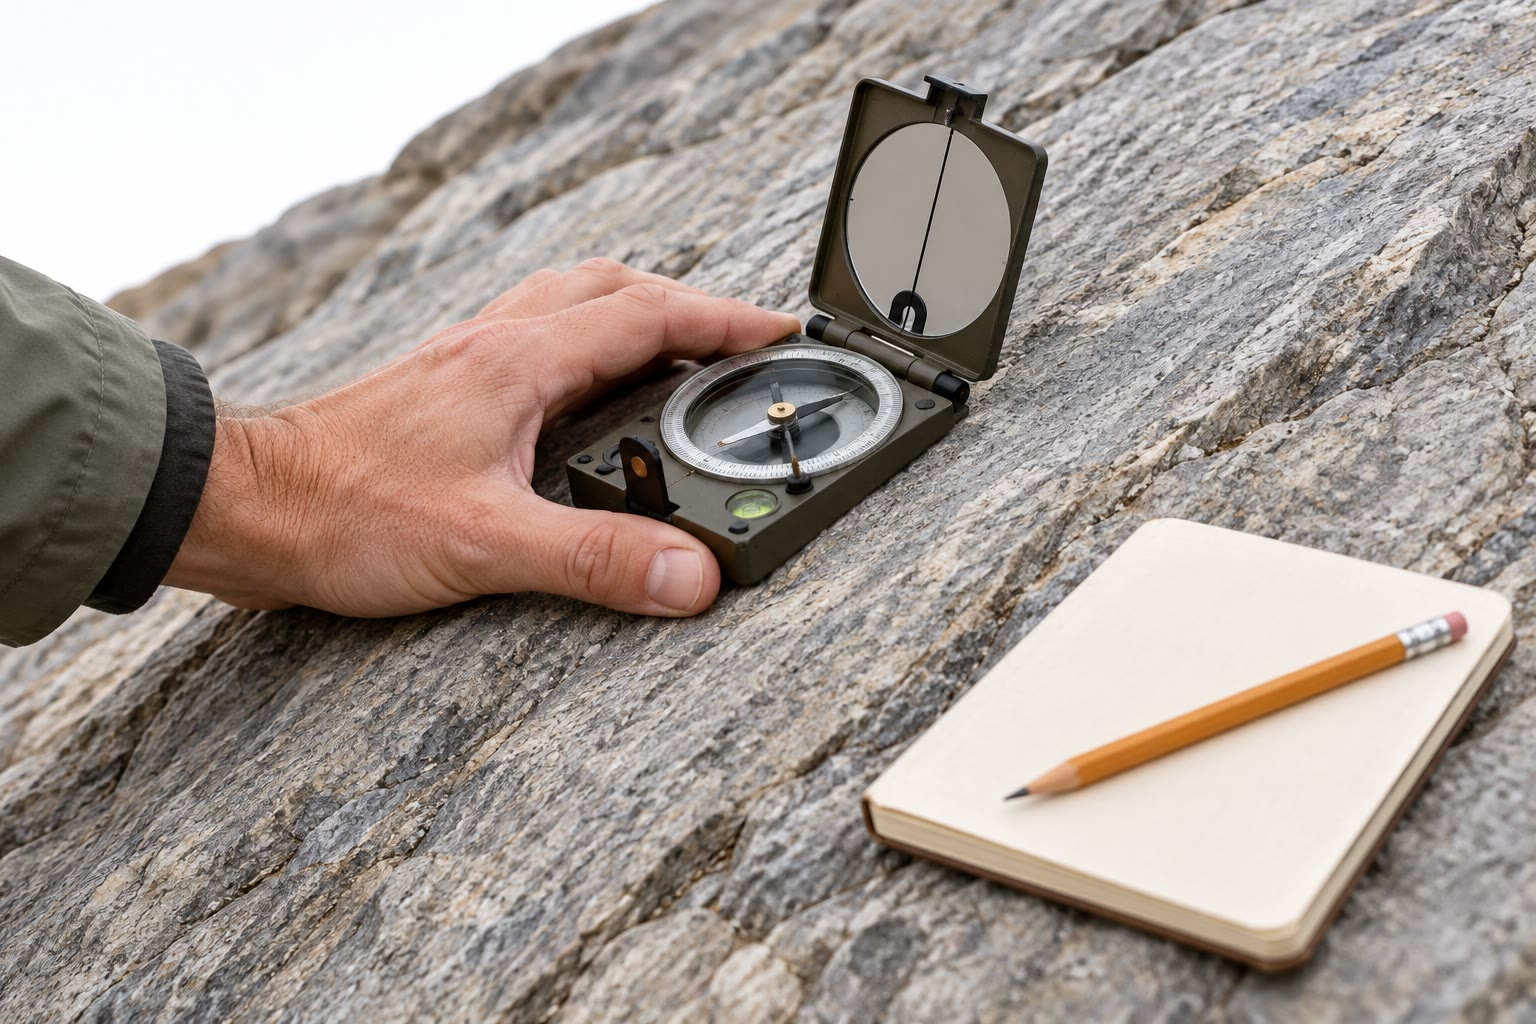
\includegraphics[width=\linewidth]{images/book5/ai/b3-compass-clinometer.jpg}

{\scriptsize Brújula-clinómetro apoyada contra una superficie rocosa inclinada, junto con una
libreta de campo (ilustración generada por IA).}
\end{minipage}
\end{inthefield}

\section{Ejercicios}

\begin{exercise}[$\star$]\label{exo:b3:structural-analysis:1}
Dedúzcanse la dirección de inmersión y la inmersión del \omterm{def:b3:structural-analysis:stereo}{polo} del plano $040/30$ (dirección de
buzamiento). Indíquese la actitud del plano cuyo \omterm{def:b3:structural-analysis:stereo}{polo} tiene dirección \ang{315} e inmersión
\ang{20}.
\end{exercise}

\begin{exercise}[$\star$]\label{exo:b3:structural-analysis:2}
Una línea tiene inmersión \ang{30}. ¿A qué distancia del centro se representa en una
\omterm{def:b3:structural-analysis:stereo}{red equiangular} y en una red equivalente, ambas de radio \qty{10}{cm}?
\end{exercise}

\begin{exercise}[$\star$]\label{exo:b3:structural-analysis:3}
Los flancos de un pliegue tienen las actitudes $090/30$ y $270/30$. Calcúlese el
ángulo entre sus \omterm{def:b3:structural-analysis:stereo}{polos} con el producto escalar de las normales, el ángulo entre flancos y
la clase del pliegue.
\end{exercise}

\begin{exercise}[$\star$]\label{exo:b3:structural-analysis:4}
Una falla $090/60$ presenta estrías de cabeceo \ang{-45}. Con el vector de rumbo
$\vec s = (0, 1, 0)$ y el vector de máxima pendiente $\vec d$ del plano, el deslizamiento
del bloque superior es $\vec u = \cos r\,\vec s - \sin r\,\vec d$. Calcúlense
$\vec d$, $\vec u$, y la dirección y la inmersión del deslizamiento. Dénse el nombre de la falla.
\end{exercise}

\begin{exercise}[$\star\star$]\label{exo:b3:structural-analysis:5}
Los flancos de un pliegue tienen las actitudes $060/40$ y $250/30$. Calcúlense la
dirección y la inmersión de su eje, y su ángulo entre flancos.
\end{exercise}

\begin{exercise}[$\star\star$]\label{exo:b3:structural-analysis:6}
Calcúlese la fracción del área de la red que queda dentro del círculo de
líneas con inmersión mayor que \ang{60}, en la red equivalente y en la \omterm{def:b3:structural-analysis:stereo}{red equiangular},
y la fracción de las direcciones del hemisferio inferior que tienen inmersión mayor
que \ang{60}. ¿Qué red debe usarse para contar \omterm{def:b3:structural-analysis:stereo}{polos}?
\end{exercise}

\begin{exercise}[$\star\star$]\label{exo:b3:structural-analysis:7}
Tres \omterm{def:b3:structural-analysis:stereo}{polos} están en el plano vertical este--oeste, a \ang{-20}, $0$ y
\ang{20} de la vertical: $\vec p = (\sin a, 0, -\cos a)$. Calcúlense su \omterm{def:b3:structural-analysis:orientation-tensor}{tensor de orientación},
sus valores propios y vectores propios, y el \omterm{def:b3:structural-analysis:pi}{eje beta}. ¿Por qué
el menor valor propio es exactamente cero?
\end{exercise}

\begin{exercise}[$\star\star$]\label{exo:b3:structural-analysis:8}
Represéntese en el diagrama de Flinn el elipsoide $X : Y : Z = 3 : 1.5 : 1$, y después el
elipsoide de volumen constante con $X = 1.8$ e $Y = 1.1$. Calcúlese $k$ en
cada caso y dénse el nombre de la deformación.
\end{exercise}

\begin{exercise}[$\star\star$]\label{exo:b3:structural-analysis:9}
En una sección cortada paralelamente al estiramiento, los ooides inicialmente redondos son
elipses de razón axial $2.25$, todas paralelas, y el área de cada una
no cambia. Calcúlense los estiramientos principales y la extensión a lo largo del eje
largo. Antes de la deformación, los centros de los ooides nunca estaban más cerca que
\qty{0.4}{mm}: dénse los semiejes del vacío del diagrama de Fry.
\end{exercise}

\begin{exercise}[$\star\star\star$]\label{exo:b3:structural-analysis:10}
Con $\theta = \ang{60}$ desde el nadir, calcúlese el estiramiento a lo largo del radio,
$\mathrm dr/(R\,\mathrm d\theta)$, y alrededor del círculo, $r/(R\sin\theta)$,
en ambas proyecciones. Compruébese el teorema sobre las proyecciones, y dése la razón
de los ejes del óvalo en que la red equivalente convierte un círculo muy pequeño
situado allí.
\end{exercise}

\begin{exercise}[$\star\star\star$]\label{exo:b3:structural-analysis:11}
En un régimen de desgarre, $\sigma_1$ es horizontal hacia \ang{000},
$\sigma_3$ horizontal hacia \ang{090} y $\sigma_2$ vertical. Una falla vertical tiene rumbo
\ang{020}. Sin calcular $\vec\tau$, muéstrese que su deslizamiento es horizontal para todo
$\Phi$. Después calcúlese $-\vec\tau$ para $\Phi = 0.4$ con
la normal del plano $\vec n = (\cos\ang{20}, -\sin\ang{20}, 0)$ y dése el
sentido del deslizamiento.
\end{exercise}

\begin{exercise}[$\star\star\star$]\label{exo:b3:structural-analysis:12}
Una sección de \qty{20}{km} de longitud corta un tren de pliegues de despegue. Dos horizontes
separados \qty{1.0}{km} se sitúan por encima de sus niveles originales en las áreas
\qty{6.0}{km^2} (inferior) y \qty{7.5}{km^2} (superior). Calcúlense el acortamiento,
la profundidad del despegue bajo el horizonte inferior, la longitud original de la
sección y su cambio relativo de longitud.
\end{exercise}

\section{Problema: pliegues y fallas de las Varden Hills}

\begin{problem}[{Problema de fin de semana --- el eje de un pliegue, el esfuerzo de un conjunto de fallas
y la restauración de una sección, en una región inventada}]
\label{pb:b3:structural-analysis:1}
% values: calc/ch08.py; figdata/bachelor-3/stereonet.py (data invented from region.py)
En las Varden Hills, la región inventada de la serie, una cobertera mesozoica descansa sobre un
zócalo de esquistos y granito. La cobertera se pliega en un anticlinal
y un sinclinal de flancos rectos, con plano axial vertical, y luego la corta una falla normal. Un
geólogo midió doce planos de estratificación en los dos flancos del anticlinal
(dirección de buzamiento/buzamiento, en grados):

\begin{center}
\small
\begin{tabular}{l|cccccc}
\hline
flanco oriental & 075/13 & 084/11 & 089/13 & 079/14 & 086/12 & 072/11 \\
flanco occidental & 283/11 & 272/13 & 281/14 & 288/10 & 276/13 & 274/12 \\
\hline
\end{tabular}
\end{center}

Las sumas de las normales unitarias hacia arriba de las seis medidas de cada flanco son
$\vec S_E = (1.2583, 0.2017, 5.8604)$ y $\vec S_W = (-1.2445, 0.1886,
5.8636)$ (este, norte, arriba). Cinco fallas llevan estrías (dirección de buzamiento/buzamiento,
cabeceo del deslizamiento del bloque superior): $120/60/{-90}$ (la falla principal), $150/55/{-76}$,
$090/65/{-108}$, $200/70/{-78}$ y $060/50/{-105}$. La falla principal tiene un
salto vertical de \qty{200}{m}. Los ejes del anticlinal y del sinclinal distan \qty{4}{km},
de modo que los pliegues se repiten cada \qty{8}{km} de este a oeste.

\medskip\noindent\textbf{Parte I --- Polos y el eje beta.}
\begin{enumerate}
  \item Indíquese la dirección y la inmersión del \omterm{def:b3:structural-analysis:stereo}{polo} de la medida $075/13$, y
        su distancia al centro de una red equivalente de radio
        \qty{10}{cm}.
  \item Calcúlese la normal unitaria hacia arriba de la medida $075/13$; compruébese
        su módulo frente a $\vec S_E$.
  \item Calcúlese la orientación media de cada flanco a partir de $\vec S_E$ y $\vec S_W$,
        las longitudes medias de la resultante y la dispersión cuadrática media de las
        medidas respecto de sus medias.
  \item Calcúlese $\vec S_E\times\vec S_W$, y la dirección y la inmersión del
        \omterm{def:b3:structural-analysis:pi}{eje beta}.
  \item Calcúlese el ángulo entre las dos normales medias, el ángulo entre flancos,
        y la clase del pliegue.
  \item El plano axial de este pliegue simétrico contiene al \omterm{def:b3:structural-analysis:pi}{eje beta} y es
        perpendicular a $\vec m_E - \vec m_W$, la diferencia de las normales unitarias
        medias. Indíquese su orientación; ¿es el pliegue vertical?
  \item Indíquese la orientación del cinturón $\pi$, y explíquese por qué los \omterm{def:b3:structural-analysis:stereo}{polos} yacen
        sobre él.
\end{enumerate}

\medskip\noindent\textbf{Parte II --- El tensor de orientación.}
El \omterm{def:b3:structural-analysis:orientation-tensor}{tensor de orientación} de los doce \omterm{def:b3:structural-analysis:stereo}{polos} es
\[
  T = \begin{pmatrix} 0.04400 & 0.00035 & 0.00109\\ 0.00035 & 0.00144 & 0.03179\\
  0.00109 & 0.03179 & 0.95456 \end{pmatrix},
\]
con los autovalores $0.95562$, $0.04400$ y $0.00038$.
\begin{enumerate}[resume]
  \item Compruébese que la traza de $T$ es 1. Con $\vec b = (0.0053, -0.9994,
        0.0333)$, el vector unitario en la dirección de $\vec S_E\times\vec S_W$, calcúlese
        $\vec b^{\mathsf T}T\vec b$. ¿Qué indica el resultado sobre $\vec b$?
  \item Calcúlese el ángulo cuadrático medio entre los \omterm{def:b3:structural-analysis:stereo}{polos} y el cinturón.
  \item Explíquese el valor de $\lambda_2$ a partir de los buzamientos de los flancos.
  \item ¿Es el pliegue cilíndrico dentro de la precisión de las medidas?
  \item La inmersión del \omterm{def:b3:structural-analysis:pi}{eje beta} viene fijada por la inclinación norte--sur del
        cinturón, al que cada \omterm{def:b3:structural-analysis:stereo}{polo} contribuye con la dispersión hallada en
        la pregunta 9. Estímese el error típico de la inmersión.
\end{enumerate}

\medskip\noindent\textbf{Parte III --- El paleoesfuerzo.}
\begin{enumerate}[resume]
  \item ¿Qué tipo de falla es la falla principal? Siguiendo a Anderson, indíquense las
        direcciones de $\sigma_1$, $\sigma_2$ y $\sigma_3$.
  \item Demuéstrese, con el teorema sobre la dirección de deslizamiento, que la falla principal
        se desliza en la dirección del buzamiento para cualquier valor de $\Phi$. ¿Qué
        indica sobre $\Phi$?
  \item Para la falla $150/55$, calcúlese $\vec n$ y sus componentes $n_1 =
        \vec n\cdot\vec e_1$ y $n_2 = \vec n\cdot\vec e_2$, con $\vec e_1$
        vertical y $\vec e_2$ horizontal hacia \ang{030}.
  \item Su deslizamiento da $\vec w = \vec n\times\vec u = (0.771, 0.605, 0.198)$.
        Calcúlese $\Phi$.
  \item Las otras tres fallas pequeñas dan $\Phi = 0.294$, $0.301$ y
        $0.306$. Indíquese la media, y explíquese de dónde procede la dispersión.
  \item ¿Qué indica $\Phi = 0.3$ sobre $\sigma_2$?
  \item Calcúlense los ejes P y T de la falla principal (a \ang{45} del
        plano, en su plano de buzamiento), y compárense con $\sigma_1$ y
        $\sigma_3$.
\end{enumerate}

\medskip\noindent\textbf{Parte IV --- Restauración de una sección este--oeste.}
\begin{enumerate}[resume]
  \item Calcúlese el buzamiento aparente del flanco oriental, $080.9/12.3$, en una
        sección este--oeste.
  \item Tomando los flancos a \ang{12} en la sección, calcúlense la longitud restaurada de una
        longitud de onda del pliegue, el acortamiento y el cambio relativo
        de longitud.
  \item Calcúlese la altura de la cresta del anticlinal sobre los sinclinales y el
        área en exceso de una longitud de onda, suponiendo que los sinclinales se mantuvieron en
        el nivel original.
  \item Calcúlese la profundidad del despegue bajo el estrato plegado. ¿Pueden
        los pliegues estar despegados en la base de la cobertera, a unos pocos cientos de metros
        de profundidad?
  \item Calcúlese el salto horizontal y el deslizamiento de la falla principal en una sección según
        \ang{120}.
  \item En la sección este--oeste, calcúlense el buzamiento aparente de la falla y
        su salto horizontal aparente. ¿Qué sección debe restaurarse?
  \item ¿En qué orden se restauran la falla y los pliegues, y dónde se sitúan las
        \omterm{def:b3:structural-analysis:restoration}{líneas de anclaje}?
  \item ¿Cuál es la inmersión del eje del pliegue de Varden, obtenida a partir de las doce
        medidas?
\end{enumerate}
\end{problem}
